\subsection{Type Switch}

Functional languages use pattern matching to perform case analysis on a given 
algebraic data type. In this section we will try to generalize this construct to 
case analysis of hierarchical and extensible data types. Presence of such a
construct will allow for external function definitions by detaching a particular 
case analysis from the hierarchy it is performed on.

A \emph{class hierarchy} is a partially ordered set $(H,\subtype)$ where $H$ is a potentially open set 
of classes and $\subtype$ is a reflexive, transitive and anti-symmetric 
\emph{subtyping relation} on $H$. We use \emph{class} and \emph{type}  
interchangeably.
% as the exact distinction is not important for this discussion. 
When two classes are in a subtyping relation $D \subtype B$, the class $D$
is said to be a (possibly indirect) \emph{derived class} (or subtype) of $B$;
the class $B$ is called a (possibly indirect) \emph{base class}
(or supertype) of $D$.
 %When the transitive reduction 
%$\subtypeD$ of $\subtype$ is a function, $H$ is usually referred to as 
%\emph{hierarchy} to indicate single inheritance.

Consider a class \code{B} and a set of classes \code{Di} directly or indirectly 
inherited from it. An object is said to be of the \emph{most derived type} 
\code{D} if it was created by explicitly calling a constructor of that type.
The inheritance relation on classes induces a subtyping relation on them, which in 
turn allows objects of a derived class to be used in places where an object of a 
base class is expected. The type of variable or parameter referencing such an
object is called the \emph{static type} of the object. When object is passed by 
reference or by pointer, we might end up in a situation where the static type of an 
object is different from its most derived type, with the latter necessarily 
being a subtype of the former. The most derived class along with all its base classes 
that are not base classes of the static type are typically referred to as the 
\emph{dynamic types} of an object. At each program point the compiler knows the 
static type of an object, but not its dynamic types.

%This section generalizes pattern matching of closed algebraic datatype values
%to case analysis of hierarchical and extensible datatype values.
In general, a \emph{type switch} or \emph{typecase} is a multiway branch statement 
that distinguishes values based on their type. In a multi-paradigm programming 
language like \Cpp{}, which supports parametric, ad-hoc, and 
subtyping polymorphisms, such a broad definition subsumes numerous different
typecase constructs studied in the literature~\cite{Intensional95,Glew99,OpenShutTypecase05}. 
In this work, we only look at typecasing scenarios based on the class inheritance 
of \Cpp{}, similar to those studied by Glew~\cite{Glew99}. 
% It is possible to generalize type switch
% (the notion, not our implementation) to static polymorphism of \Cpp{} (ad-hoc and 
% parametric polymorphism enabled by overloading and templates) along the line of 
% work introduced by Harper and Morrisett~\cite{Intensional95} and studied in the
% context of closed and extensible solutions by Vytiniotis et 
% al~\cite{OpenShutTypecase05}, but we do not address such a generalization here.
We use the term \emph{type switch} instead of a broader \emph{typecase} to 
stress the run-time nature of the type analysis similar to how regular 
\code{switch}-statement of \Cpp{} performs case analysis of values at run time.

The term \emph{object descriptor} means either a pointer or a reference to 
an object.
Given an object descriptor, called \emph{subject}, of static type \code{S} 
referred to as the \emph{subject type}, and a list of 
\emph{target types} \code{Ti} associated with the branches, a type switch 
statement needs to identify a suitable clause $m$ based on 
the dynamic type \code{D <: S} of the subject as well as a suitable 
conversion that coerces the subject to the target type \code{Tm}.  
Due to multiple inheritance, types \code{Ti} may not all directly
derive from the static type \code{S}. However,
%because of the strong static type safety requirement, 
the type of the applicable clause \code{Tm} will necessarily have to be a 
supertype of the subject's dynamic type \code{D <: Tm}. 
A hypothetical type switch 
statement, not currently supported by \Cpp{}, may look as following:
%
\begin{lstlisting}
switch (subject)
{
    case T1: s1;
    ...
    case Tn: sn;
}
\end{lstlisting}
%
\noindent
There is no need for an explicit \emph{default clause} in our setting because 
it is semantically equivalent to a case clause guarded by the 
subject type: \code{case S: s}. The only semantic difference such a choice 
makes is in the treatment of null pointers.
One may naively think that null pointers should be handled by
the default clause.  However, not distinguishing between 
invalid object and valid object of a known static but unknown dynamic type may 
lead to nasty run-time errors.

%\noindent
Similar control structures exist in many programming languages, e.g. 
\emph{match} in Scala~\cite{Scala2nd}, \emph{case} in Haskell~\cite{Haskell98Book} and 
ML~\cite{ML90}, \emph{typecase} in Modula-3~\cite{Modula3TS} and CLOS (as a 
macro), \emph{tagcase} in CLU~\cite{CLURefMan}, \emph{union case} in Algol 68, 
and date back to at least Simula's \emph{Inspect} statement~\cite{Simula67}. 
The statement can, in general, be given numerous plausible semantics:
%
\begin{itemize}
\setlength{\itemsep}{0pt}
\setlength{\parskip}{0pt}
\item \emph{First-fit} semantics will evaluate the first statement $s_i$ such 
      that $T_i$ is a base class of $D$.
\item \emph{Best-fit} semantics will evaluate the statement corresponding to the 
      most-specialized base class $T_i$ of $D$ if it is unique (subject to 
      ambiguity).
\item \emph{Exact-fit} semantics will evaluate statement $s_i$ if $T_i=D$.
\item \emph{All-fit} semantics will evaluate all statements $s_i$ whose guard 
      type $T_i$ is a supertype of $D$ (order of execution has to be defined).
\item \emph{Any-fit} semantics might choose non-deterministically one of the 
      statements enabled by the all-fit semantics.
\end{itemize}
%
The list is not exhaustive and depending on a language, any of them
is a plausible choice. Functional languages, for example, often prefer 
first-fit semantics because it is similar to case analysis in mathematics. 
Object-oriented languages are typically inclined to best-fit semantics due 
to its similarity to overload resolution and run-time dispatch; however, some 
do opt for first-fit semantics to mimic the functional style: e.g. Scala~\cite{Scala2nd}. 
Exact-fit semantics can often be seen in languages supporting discriminated 
union types (sum types): e.g. \emph{variant records} in Pascal, Ada and Modula-2, 
\emph{oneof} and \emph{variant objects} in CLU, \emph{unions} in C and \Cpp{}, etc. 
All-fit and any-fit semantics might be seen in languages based on predicate 
dispatching~\cite{ErnstKC98} or guarded commands~\cite{EWD:EWD472}, where a 
predicate can be seen as a characteristic function of a type, while logical 
implication can be seen as subtyping.

\subsection{Open and Efficient Type Switching}
\label{sec:poets}

The fact that algebraic data types in functional languages are closed allows for 
their efficient implementation. The traditional compilation scheme assigns unique 
tags to every variant of the algebraic data type and pattern matching is then 
simply implemented with a jump table over all tags. A number of issues in 
object-oriented languages makes this extremely efficient approach infeasible:

\begin{itemize}
\setlength{\itemsep}{0pt}
\setlength{\parskip}{0pt}
\item Extensibility
\item Subtyping
\item Multiple inheritance
\item Separate compilation
\item Dynamic linking 
\end{itemize}

\noindent
Unlike functional style algebraic data types, classes are \emph{extensible} 
whereby new variants can be arbitrarily added to the base class in the form of 
derived classes. Such extension can happen in a different translation unit or a
static library (subject to \emph{separate compilation}) or a dynamically linked 
module (subject to \emph{dynamic linking}). Separate compilation effectively 
implies that all the derived classes of a given class will only be known at link 
time, postponing thus any tag-allocation related decisions until then. The 
Presence of dynamic linking effectively requires the compiler to assume that the 
exact derived classes will only be known at run time, and not even at start-up 
time.

%and thus any tag allocation scheme should on one hand assume presence of 
%unknown tags and on the other -- the necessity of maintaing the same tags for 
%the commonly seen classes of each dynamic module.  

The \emph{subtyping} relation that comes along with extensibility through 
subclassing effectively gives every class multiple types -- its own and the 
types of all its base classes. In such a scenario it is natural to require that 
type switching can be done not only against the exact dynamic type of an object, 
but also against any of its base classes (subject to our substitutability 
requirement). This in itself is not a problem for functional-style tag 
allocation as long as the set of all derived classes is known, since the 
compiler can partition tags of all the derived classes according to chosen 
semantics based on classes mentioned in case clauses.
Unfortunately this will not work in the presence of dynamic linking as there 
might be new derived classes with tags not known at the time of partitioning and 
thus not mentioned in the generated jump table.

\emph{Multiple inheritance} complicates things further by making each class 
potentially belong to numerous unrelated hierarchies. Any tag allocation scheme 
capable of dealing with multiple inheritance will either have to assure that 
generated tags satisfy properties of each subhierarchy independently or use 
different tags for different subhierarchies. Multiple inheritance also 
introduces such a phenomenon as \emph{cross-casting}, whereby a user may request 
to cast pointers between unrelated classes, since they can potentially become 
base classes of a later defined class. From an implementation point of view this 
means that not only do we have to be able to check that a given object belongs 
to a given class (type testing), but also be able to find a correct offset to it 
from a given base class (type casting).

While looking at various schemes for implementing type switching we noted down a 
few questions that might help evaluate and compare solutions: 

\begin{enumerate}
\setlength{\itemsep}{0pt}
\setlength{\parskip}{0pt}
\item Can the solution handle base classes in case clauses?
\item Will it handle the presence of base and derived classes in the same match statement?
\item Will it work with derived classes coming from a DLL?
\item Can it cope with multiple inheritance (repeated, virtual)?
\item Can independently developed DLLs that either extend classes involved in 
      type switching or do type switching themselves be loaded together without 
      any integration efforts?
\item Are there any limitations on the number and or shape of class extensions?
\item What is the complexity of performing matching, based on the number of case clauses and 
      the number of possible types?
\end{enumerate}

The number of possible types in the last question refers to the number of subtypes 
of the static type of the subject, not all the types in the program. Several 
solutions discussed below depend on the number of case clauses in the match 
statement, which raises the question of how many such clauses a typical program 
might have. The C++ pretty-printer for Pivot we implemented using our pattern 
matching techniques originally had 8 match statements with 5, 7, 8, 10, 15, 17, 30 
and 63 case clauses each. While experimenting 
with probability distributions of various classes to minimize the number of 
conflicts (see \textsection\ref{sec:moc}), we had to associate probabilities 
with classes and implemented it with a match statement over all 160 nodes in the 
Pivot's class hierarchy. With Pivot having the smallest number of node kinds 
among the compiler frameworks we had a chance to work with, we expect a similar 
or larger number of case clauses in other compiler applications.

\subsection{An Open Type Switch}

Type switch alone does not solve the expression problem in the context
of an object-oriented language, for the existing code may have to be 
modified to consider new variants. Relying on a default clause is not 
an acceptable solution in this situation, because often the 
only reasonable default behavior is to raise an exception. 
Zenger and Odersky observed that defaults transform type errors that should
manifest statically into runtime exceptions~\cite{fool12}.
In our experience, newly added variants were more often extending an existing 
variant than creating an entirely disjoint one. In a compiler, for 
example, a new kind of type expression will typically extend a 
\code{TypeExpression} variant, while a new form of annotation will extend an 
\code{Annotation} variant, thus not extending the root \code{ASTNode} directly. 
Due to the substitutability requirement, this new variant will be treated as a 
variant it extends in all the existing code. The functions that will be affected 
by its addition and thus have to be modified will be limited to functions 
directly analyzing the variant it extends and not providing a default behavior.

To account for this subtlety of extensible hierarchical data types, we use a 
term \emph{open type switch} to refer to a type switch that satisfies all the 
requirements of an \emph{open solution to the expression problem} stated above 
except for the \emph{no modification or duplication} requirement. We loosen it 
to allow modification of functions for which the newly added variant becomes a 
disjoint (orthogonal) case not handled by a default clause. We believe that the 
loosened requirement allows us to express pragmatically interesting restrictions 
that developers are willing to live with. Furthermore, 
open type switch overcomes 
all the major shortcomings of the visitor design pattern:
%
\begin{itemize}
\setlength{\itemsep}{0pt}
\setlength{\parskip}{0pt}
\item Case analysis with an open type switch is non-intrusive as it 
      inspects the hierarchy externally and can be applied retroactively. 
\item New variants can be accounted for in the newly written code and will be 
      seen as a base class or default in the existing code.
\item The affected functions are limited to those for which the newly added 
      variant is a disjoint case.
\item The code avoids the control inversion and the need for boilerplate code 
      that visitors introduce, and is thus a more direct expression of the 
      intent.
\end{itemize}

\subsection{\Cpp{} Specifics: Subobjects}
\label{sec:specifics}

\Cpp{} supports two kinds of multiple inheritance: 
\emph{non-virtual} inheritance and \emph{virtual} inheritance~\cite{CPPARM90}. 
The difference between the two only arises in situations where a 
class indirectly inherits from the same base class via more than one path
in its class hierarchy.  Rigorous accounts of \Cpp{} multiple inheritance
semantics use the notion of \emph{subobject}~\cite{RF95}.

\begin{figure}[htbp]
  \centering
    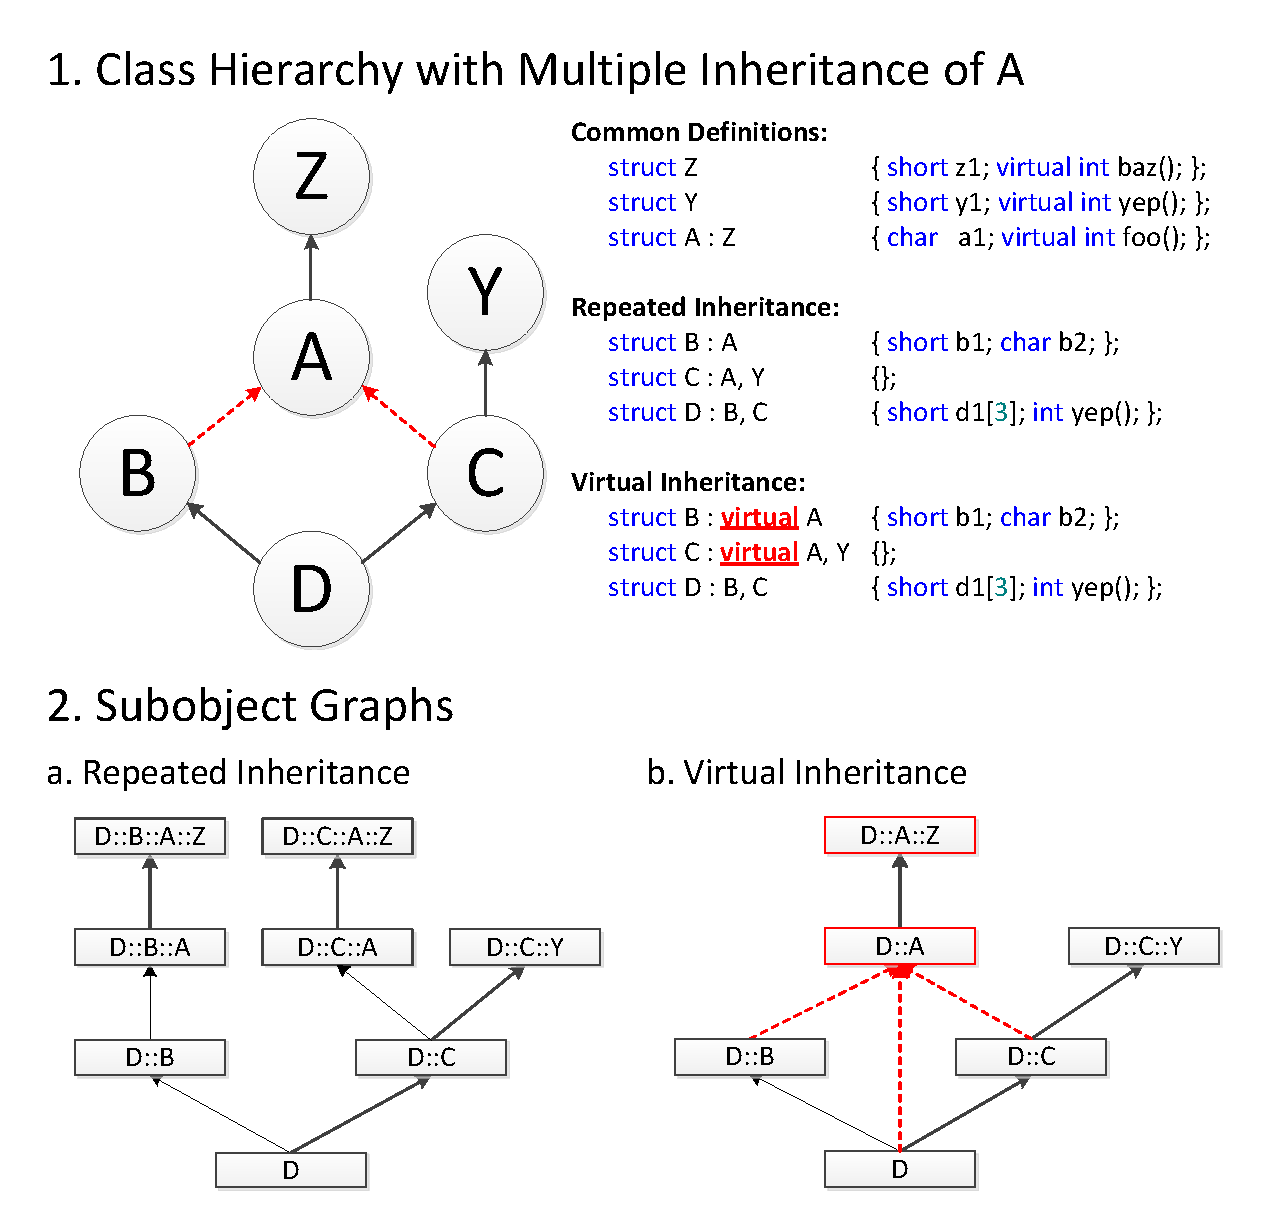
\includegraphics[width=0.47\textwidth]{Inheritance.pdf}
  \caption{Multiple Inheritance in \Cpp{}}
  \label{fig:inheritance}
\end{figure}

\noindent
Consider the simple class hierarchy in Figure~\ref{fig:inheritance}(1). Class 
\code{D} indirectly inherits from class \code{A} through its \code{B} and 
\code{C} base classes. In this case, the user may opt to keep distinct 
subobjects of class \code{A} (repeated inheritance) or a shared one (virtual 
inheritance) by specifying how \code{B} and \code{C} inherit from 
\code{A}. The kind of inheritance is thus not a property of a given class, but a 
property of an inheritance relation between classes and it is possible to mix the two. 

A class hierarchy gives rise to a \emph{subobject graph}, where a given class 
node may be replicated when inherited repeatedly or left shared when inherited 
virtually. The edges in such a graph represent \emph{subobject containment} and 
indicate whether such containment is shared or exclusive. 
Every class $C$ in the class hierarchy will have its own subobject 
graph representing the subobjects of an object of dynamic type $C$.
Figure~\ref{fig:inheritance}(2) shows subobject graph for class \code{D} 
obtained for the class hierarchy in Figure~\ref{fig:inheritance}(1) under repeated (a) and virtual (b) 
inheritance of class \code{A} by classes \code{B} and \code{C}. The shared 
containment is indicated with the dashed arrows, while exclusive -- with the solid 
ones.

\Cpp{}'s notion of multiple inheritance is fundamentally about 
subobjects, not just types.  Virtual inheritance is about
sharing the base-class subobjects, whereas non-virtual inheritance
reflects distinction in base-class subobjects from distinct class inheritance paths~\cite{CPPARM90}.

An object descriptor of static type $A$ referencing an object of the dynamic 
type $C$ can be understood as any $C$\code{::*::}$A$-node in the subobject graph of $C$. 
Casts can be understood as a change from one subobject to another.
We use the terms \emph{source subobject} and \emph{target 
subobject} to refer to the argument and result of the cast, respectively. Their 
static types will be referred to as \emph{source type} and \emph{target type} 
respectively. \Cpp{} distinguishes three kinds of casts: upcasts, downcasts, and 
crosscasts.

An \emph{upcast} is a cast from a derived class to one of its bases. When the 
base class is unambiguous, such casts are implicit and require no additional 
annotations. When the base class is ambiguous, cast failure is manifested 
statically in the form of a compile-time error. For example, this is the case with 
casting \code{D} to \code{A} under repeated multiple inheritance of \code{A}, 
in which case the user needs to explicitly cast the object to \code{B} or 
\code{C} first in order to indicate the desired subobject and resolve the ambiguity. 
In some cases, however, introduction of such an explicit cast is not possible: 
e.g. in implicit conversions generated by the compiler to implement covariant 
return types, crosscasts or conversions in generic code. This does not mean 
that in such cases we violate the Liskov substitution principle: the 
classes are still in a subtyping relation, but an implicit conversion is not 
available.

A \emph{downcast} is a cast from a base class to one of its derived classes. The 
cast has to determine at run-time whether the source subobject is contained by a 
subobject of the target type in the dynamic type's subobject graph. Failure 
of such a cast is manifested dynamically at run-time.

A \emph{crosscast} is a cast between classes that are not necessarily related by 
inheritance except by sharing a common derived class (subclass).
Accordingly to the \Cpp{} semantics such cast is defined to be a 
composition of upcast to target type and downcast to the dynamic type. 
While the downcast to the dynamic type is always guaranteed to succeed 
regardless of the source subobject, the upcast to the target type may be 
ambiguous, in which case the cast will fail at runtime. A cast from \code{Y} to 
\code{B} inside an object of dynamic type \code{D} in 
Figure~\ref{fig:inheritance}(2a,2b) is an example of a successful crosscast. A 
similar cast from \code{Y} to \code{A} inside \code{D} under the repeated  
inheritance in Figure~\ref{fig:inheritance}(2a) will fail because of the ambiguous 
upcast from \code{D} to \code{A}.

An interesting artifact of these distinctions can be seen in an example of 
casting a subobject of type \code{Z} to a subobject of type \code{A} in 
Figure~\ref{fig:inheritance}(2a). The subobject \code{D::B::A::Z} will be 
successfully cast to \code{D::B::A}, while the \code{D::C::A::Z} will be 
successfully cast to \code{D::C::A}. These casts do not involve downcasting to 
\code{D} followed by an upcast to \code{A}, which would be ambiguous, but 
instead take the dynamic type of a larger subobject (\code{D::B} or \code{D::C}) 
that the source subobject is contained in into account in order to resolve the 
ambiguity. A similar cast from \code{Y} to \code{A} will fail; should 
\code{Y} have also been non-virtually derived from \code{Z}, the cast from 
\code{D::C::Y::Z} to \code{A} would have failed. This shows that the distinction 
between crosscast and downcast is not based solely on the presence of a 
subtyping relation between the source and target types, but also on the actual 
position of the source subobject in the dynamic type's subobject graph.

The \Cpp{} inheritance model, presented here informally, further complicates the definition and
implementation of a type switch compared to simpler models. We have to define the
type switch so that only unambiguous casting between a source and a target within an object is possible.
That is, the implementation of the cast between source and target subobjects must take into account the
location of the source subobject in the subobject graph, rather than
just the dynamic and target types, which would suffice for a simple subtype testing.
Of course, every use of dynamic casting and every implicit cast are type safe~\cite{WNST06}.

%\section{Problem Description} %%%%%%%%%%%%%%%%%%%%%%%%%%%%%%%%%%%%%%%%%%%%%%%%%%
%\label{sec:probl}

\subsection{Existing Approaches to Type Case Analysis}
\label{sec:prev}

The closed nature of algebraic data types allows for their efficient 
implementation. The traditional compilation scheme assigns unique (and often 
small and sequential) tags to every variant of the algebraic data type and type 
switching is then simply implemented with a multi-way branch~\cite{Spuler94} 
(usually a jump table) over all the tags~\cite{Augustsson85}. Dealing with 
extensible hierarchical data types makes this %extremely efficient 
approach infeasible:

\begin{itemize}
\setlength{\itemsep}{0pt}
\setlength{\parskip}{0pt}
\item \emph{Extensibility} implies that the compiler may not know the exact set 
      of all the derived classes until link-time (due to \emph{separate compilation}) 
      or even run-time (due to \emph{dynamic linking}).
\item \emph{Substitutability} implies that we should be able to 
      match tags of derived classes against case labels representing tags of 
      base classes.
\item The presence of \emph{multiple inheritance} might require pointer adjustments 
      that are not known at compile time (e.g. due to virtual base classes, 
      ambiguous base classes or crosscasting).
\end{itemize}

%\noindent
%In some cases the substitutability requirement can be satisfied by obtaining 
%the base class' tag from a derived one first and then performing the jump. 
%This will work as long as we have only base classes in the case clauses.
%Derived classes that have to be treated separately from the rest of their 
%siblings will essentially be indistinguishable from them.
%
%When tags are not chosen arbitrarily but to reflect the subtyping relation of the 
%underlying hierarchy (e.g. certain bit set for certain base class), the assumed 
%structure of tags is likely to make the set of tags sparse. On one hand this 
%decreases the number of representable hierarchies and thus hinders openness, 
%while on the other it forces the compiler to use a decision tree instead of a jump 
%table to implement the switch. The former was consistently slower than the 
%latter one in our experience, even though the opposite was noted on some 
%architectures for small number of case clauses~\cite[\textsection 4]{garrigue-98}.

\noindent
There are two main approaches to implementing case analysis on extensible 
hierarchical data types discussed in the literature.

The first approach is based on either explicit or implicit sealing of the class 
hierarchy on which type switching can be performed. \Cpp{}11, for example, allows 
the user to prohibit further derivation by specifying a class to be ``final''~\cite{C++11}, 
similar to Scala and Java. The compiler then may use the above tag 
allocation over all variants to implement type analysis~\cite[\textsection 
4.3.2]{EmirThesis}. 
In some cases, the sealing may happen implicitly. For example, languages %that allow names 
with both internal and external linkage may employ the fact that classes 
with internal linkage will not be externally accessible and are thus effectively 
sealed. While clearly efficient, the approach is not open as it avoids the 
question rather than answers it. 

The broader problem with this approach is that techniques that rely on unique or
sequential compile or link-time constants violate independent extensibility 
since without a centralized authority there is no guarantee same constant will 
not be chosen in a type-unsafe manner by independent extensions. Updating such 
constants at load time may be too costly even when possible. %More often than 
%not, however such updates may require code regeneration since decision trees, 
%lookup tables etc. may have been generated by compiler for given values.

An important practical solution that follows this approach is the visitor design 
pattern~\cite{DesignPatterns1993}. The set of \code{visit} methods in a visitor's 
interface essentially seals the class hierarchy. Extensions have been proposed 
in the literature~\cite{Zenger:2001}, but they have problems of their own, 
as discussed in \textsection\ref{sec:rw}.

The second approach employs type inclusion tests combined with decision 
trees~\cite{Cardelli84} to avoid unnecessary checks. Its efficiency is then 
entirely focused on the efficiency of type inclusion 
tests~\cite{Schubert83,Wirth88,Cohen91,Caseau93,Vortex96,Krall97nearoptimal,Vitek97,PQEncoding,FastDynCast,Ducournau08}. 

%"A couple of years later, Nikolaus With published an approach based on type 
%inclusion. However, that approach does not work well in the presence of multiple 
%inheritance and separates the single logical operation of gaining type-safe 
%access to an object into two, implying the possibility of a programmer error." 

\Cpp{} has handled general dynamic casting since 1987, when multiple inheritance 
was added to the language~\cite{Str87}. Wirth later presented a technique that 
can be used to implement subtype tests by traversing a linked list of 
types~\cite{Wirth88}. His encoding required little space, but ran in time 
proportional to the distance between the two types in the class hierarchy. 
A trivial constant-time type inclusion test can be implemented with a 
\emph{binary matrix}, encoding the subtyping relation on the class 
hierarchy~\cite{Vortex96}. While efficient in time, it has quadratic space 
requirements, which makes it expensive for use on large class hierarchies. Cohen 
proposed the first space-efficient constant-time algorithm, but it can
only deal with single inheritance~\cite{Cohen91}. \emph{Hierarchical encoding} 
is another constant-time test that maps subtype queries into subset queries on 
bit-vectors~\cite{Caseau93,Krall97nearoptimal}. The approach can handle multiple
inheritance, but the space and time required for a subtype test in this encoding 
increases with the size of the class hierarchy; also, Caseau's approach~\cite{Caseau93} is 
limited to class hierarchies that are lattices. Schubert's \emph{relative 
numbering}~\cite{Schubert83} encodes each type with an interval $[l,r]$, 
effectively making type inclusion tests isomorphic to a simple range checking. 
The encoding is optimal in space and time, but it is limited to single 
inheritance. \emph{PQ-Encoding} of Zibin and Gil employs PQ-trees to improve 
further space and time efficiency of the constant-time inclusion 
testing~\cite{PQEncoding}. While capable of handling type inclusion queries on 
hierarchies with multiple inheritance, the approach makes the closed world assumption and can be costly 
for use with dynamic linking because it is not incremental.
The approach of Gibbs and Stroustrup~\cite{FastDynCast} employs divisibility of 
numbers to obtain a constant-time type inclusion test. The approach can handle 
multiple inheritance and was the first constant-time technique to addresses the 
problem of casts between subobjects. Unfortunately, the approach limits the size 
of the class hierarchies that can be encoded with this technique. 
Ducournau proposed a constant-time inclusion test based on the fact that, in an 
open solution, a class has a known number of base classes, and thus perfect hashes 
can be used to map them to this-pointer offsets typically used to implement 
subobject casts \cite{Ducournau08}. Unfortunately, the approach addresses only 
virtual multiple inheritance and (similarly to other approaches) relies on 
load-time computations. An excellent introduction to and detailed 
analysis of existing constant-time type inclusion tests can be found in 
\cite{Vitek97,PQEncoding}.

With the exception of work by Gibbs and Stroustrup~\cite{FastDynCast}, all the 
approaches to efficient type-inclusion testing we found in the literature were 
based on the assumption that \emph{the outcome of a subtyping test as well as 
the subsequent cast depend only on the target type and the dynamic type of 
the object}. Although that assumption is sound for subtyping tests and subtype 
casts for shared inheritance (including single), it does not reflect the 
relationship between subobjects in the general case of multiple inheritance 
as found in \Cpp{}.

\subsection{The Source of Inefficiency}

While constant-time type inclusion tests are invaluable in optimizing subtype 
tests in programming languages, their use in implementing a type switch is 
inferior to some workaround techniques. This may prevent wide adoption of a 
language implementation of such a feature due to its inferior performance. 
We implemented 3 constant-time type inclusion tests: binary 
matrix~\cite{Vitek97}, Cohen's algorithm~\cite{Cohen91}, and fast dynamic 
cast~\cite{FastDynCast} and combined them with a decision tree to implement a 
type switch on a class hierarchy ideally suited for such scenarios: a perfect binary tree with 
classes number $2i$ and $2i+1$ derived from a class number $i$. Our workaround 
techniques included the visitor design pattern and a switch on the sealed sequential 
set of tags.

\begin{figure}[htbp]
  \centering
    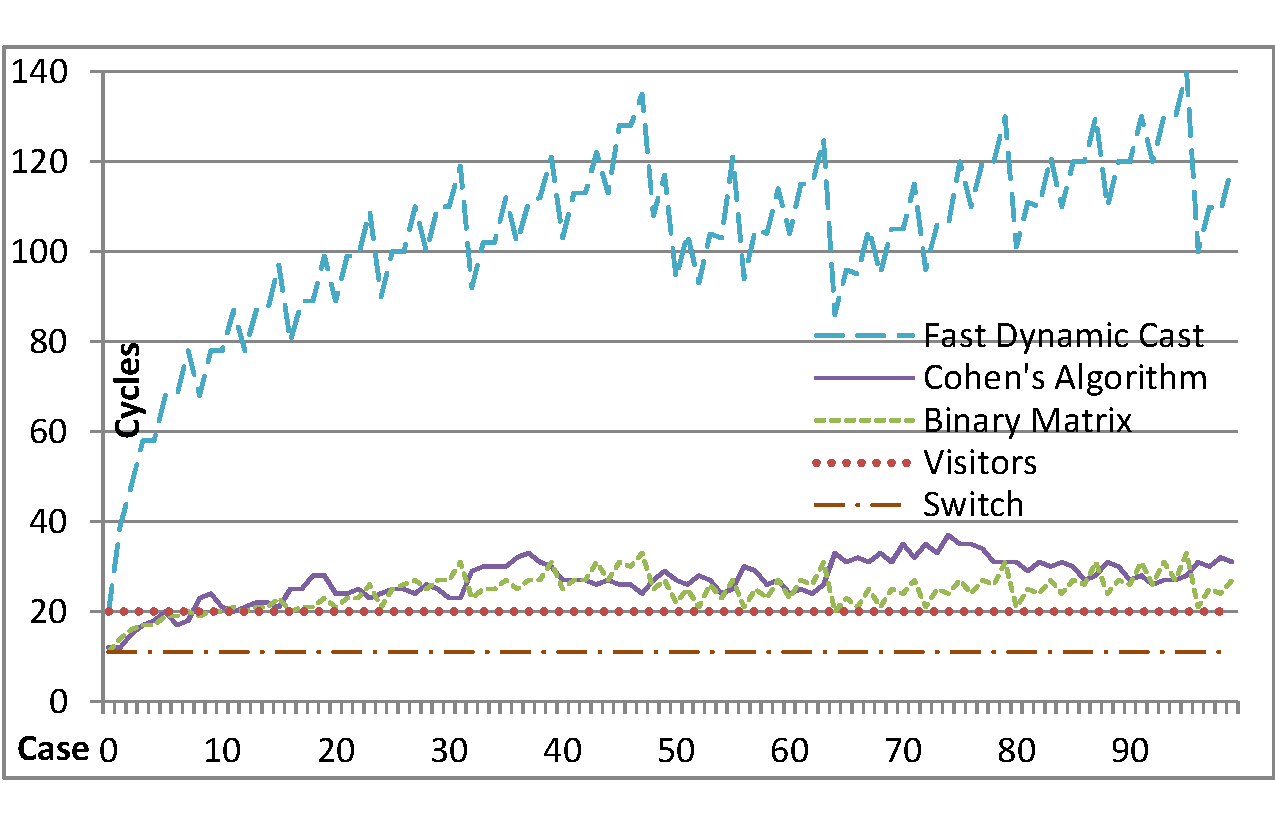
\includegraphics[width=0.47\textwidth]{DCast-vs-Visitors.pdf}
  \caption{Type switch based on constant-time subtype tests}
  \label{fig:DCastVis2}
\end{figure}

The chart in Figure~\ref{fig:DCastVis2} shows the number of cycles (Y-axis) each 
technique took to recognize an object of the dynamic type $i$ (X-axis). 
Despite known limitations, binary matrix and Cohen's algorithm are some of the 
fastest known type inclusion tests for single inheritance~\cite{Vitek97}. It 
is nonetheless easy to see that the logarithmic cost associated with the 
decision tree very quickly surpasses the constant overhead of double dispatch 
(20 cycles) present in the visitor design pattern or the jump-table 
implementation of the switch on all tags (11 cycles). We expect the cost of 
techniques capable of handling multiple inheritance to be even higher, especially 
those addressing casting between subobjects (e.g. fast dynamic cast). The edgy 
shape of timing results reflects the shape of the class hierarchy used for this 
experiment.
%We show in \textsection{sec:viscmp} that 
%our open solution is capable of delivering an amortized constant-time type 
%switching wi